\documentclass[1p]{elsarticle_modified}
%\bibliographystyle{elsarticle-num}

%\usepackage[colorlinks]{hyperref}
%\usepackage{abbrmath_seonhwa} %\Abb, \Ascr, \Acal ,\Abf, \Afrak
\usepackage{amsfonts}
\usepackage{amssymb}
\usepackage{amsmath}
\usepackage{amsthm}
\usepackage{scalefnt}
\usepackage{amsbsy}
\usepackage{kotex}
\usepackage{caption}
\usepackage{subfig}
\usepackage{color}
\usepackage{graphicx}
\usepackage{xcolor} %% white, black, red, green, blue, cyan, magenta, yellow
\usepackage{float}
\usepackage{setspace}
\usepackage{hyperref}

\usepackage{tikz}
\usetikzlibrary{arrows}

\usepackage{multirow}
\usepackage{array} % fixed length table
\usepackage{hhline}

%%%%%%%%%%%%%%%%%%%%%
\makeatletter
\renewcommand*\env@matrix[1][\arraystretch]{%
	\edef\arraystretch{#1}%
	\hskip -\arraycolsep
	\let\@ifnextchar\new@ifnextchar
	\array{*\c@MaxMatrixCols c}}
\makeatother %https://tex.stackexchange.com/questions/14071/how-can-i-increase-the-line-spacing-in-a-matrix
%%%%%%%%%%%%%%%

\usepackage[normalem]{ulem}

\newcommand{\msout}[1]{\ifmmode\text{\sout{\ensuremath{#1}}}\else\sout{#1}\fi}
%SOURCE: \msout is \stkout macro in https://tex.stackexchange.com/questions/20609/strikeout-in-math-mode

\newcommand{\cancel}[1]{
	\ifmmode
	{\color{red}\msout{#1}}
	\else
	{\color{red}\sout{#1}}
	\fi
}

\newcommand{\add}[1]{
	{\color{blue}\uwave{#1}}
}

\newcommand{\replace}[2]{
	\ifmmode
	{\color{red}\msout{#1}}{\color{blue}\uwave{#2}}
	\else
	{\color{red}\sout{#1}}{\color{blue}\uwave{#2}}
	\fi
}

\newcommand{\Sol}{\mathcal{S}} %segment
\newcommand{\D}{D} %diagram
\newcommand{\A}{\mathcal{A}} %arc


%%%%%%%%%%%%%%%%%%%%%%%%%%%%%5 test

\def\sl{\operatorname{\textup{SL}}(2,\Cbb)}
\def\psl{\operatorname{\textup{PSL}}(2,\Cbb)}
\def\quan{\mkern 1mu \triangleright \mkern 1mu}

\theoremstyle{definition}
\newtheorem{thm}{Theorem}[section]
\newtheorem{prop}[thm]{Proposition}
\newtheorem{lem}[thm]{Lemma}
\newtheorem{ques}[thm]{Question}
\newtheorem{cor}[thm]{Corollary}
\newtheorem{defn}[thm]{Definition}
\newtheorem{exam}[thm]{Example}
\newtheorem{rmk}[thm]{Remark}
\newtheorem{alg}[thm]{Algorithm}

\newcommand{\I}{\sqrt{-1}}
\begin{document}

%\begin{frontmatter}
%
%\title{Boundary parabolic representations of knots up to 8 crossings}
%
%%% Group authors per affiliation:
%\author{Yunhi Cho} 
%\address{Department of Mathematics, University of Seoul, Seoul, Korea}
%\ead{yhcho@uos.ac.kr}
%
%
%\author{Seonhwa Kim} %\fnref{s_kim}}
%\address{Center for Geometry and Physics, Institute for Basic Science, Pohang, 37673, Korea}
%\ead{ryeona17@ibs.re.kr}
%
%\author{Hyuk Kim}
%\address{Department of Mathematical Sciences, Seoul National University, Seoul 08826, Korea}
%\ead{hyukkim@snu.ac.kr}
%
%\author{Seokbeom Yoon}
%\address{Department of Mathematical Sciences, Seoul National University, Seoul, 08826,  Korea}
%\ead{sbyoon15@snu.ac.kr}
%
%\begin{abstract}
%We find all boundary parabolic representation of knots up to 8 crossings.
%
%\end{abstract}
%\begin{keyword}
%    \MSC[2010] 57M25 
%\end{keyword}
%
%\end{frontmatter}

%\linenumbers
%\tableofcontents
%
\newcommand\colored[1]{\textcolor{white}{\rule[-0.35ex]{0.8em}{1.4ex}}\kern-0.8em\color{red} #1}%
%\newcommand\colored[1]{\textcolor{white}{ #1}\kern-2.17ex	\textcolor{white}{ #1}\kern-1.81ex	\textcolor{white}{ #1}\kern-2.15ex\color{red}#1	}

{\Large $\underline{11a_{85}~(K11a_{85})}$}

\setlength{\tabcolsep}{10pt}
\renewcommand{\arraystretch}{1.6}
\vspace{1cm}\begin{tabular}{m{100pt}>{\centering\arraybackslash}m{274pt}}
\multirow{5}{120pt}{
	\centering
	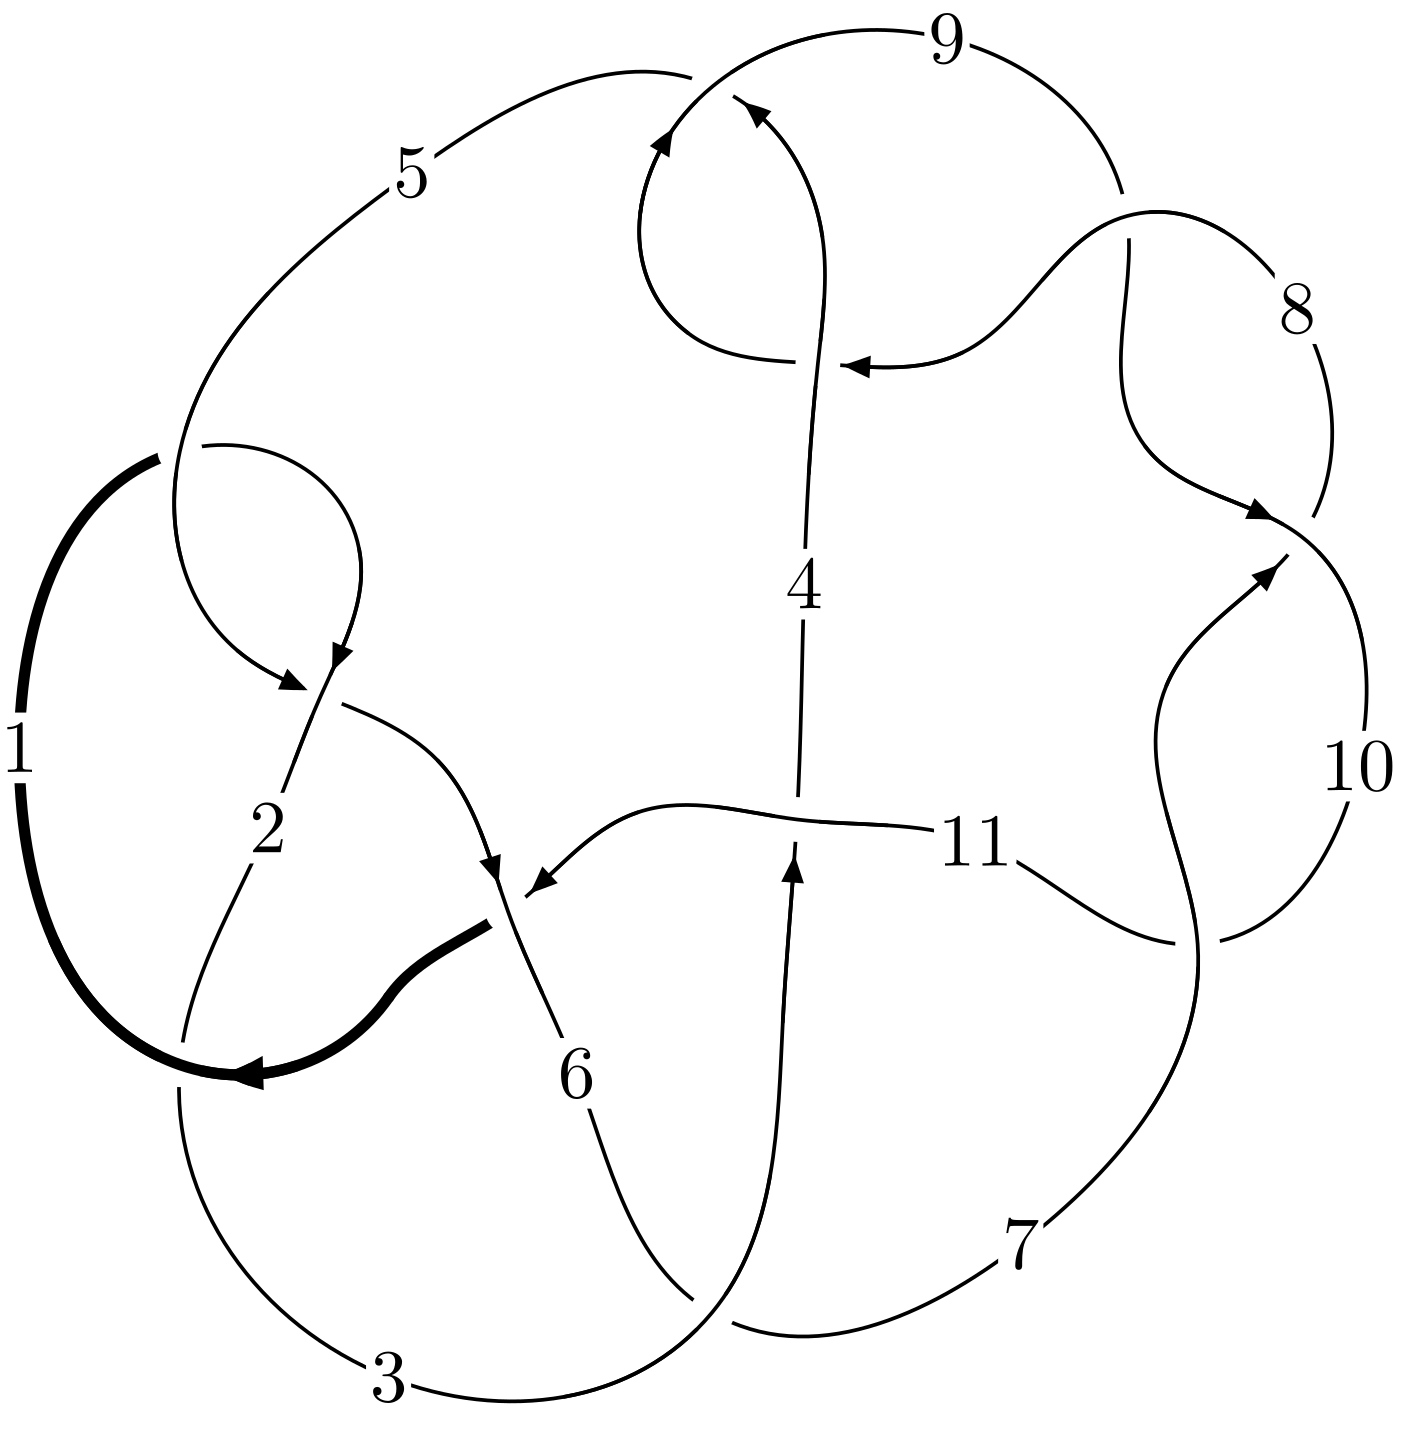
\includegraphics[width=112pt]{../../../GIT/diagram.site/Diagrams/png/334_11a_85.png}\\
\ \ \ A knot diagram\footnotemark}&
\allowdisplaybreaks
\textbf{Linearized knot diagam} \\
\cline{2-2}
 &
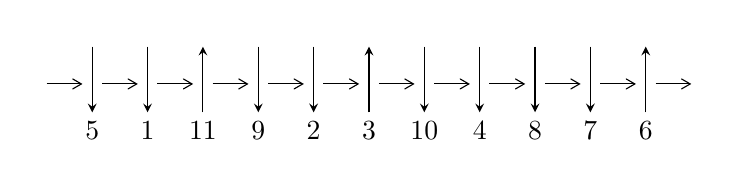
\begin{tikzpicture}[x=20pt, y=17pt]
	% nodes
	\node (C0) at (0, 0) {};
	\node (C1) at (1, 0) {};
	\node (C1U) at (1, +1) {};
	\node (C1D) at (1, -1) {5};

	\node (C2) at (2, 0) {};
	\node (C2U) at (2, +1) {};
	\node (C2D) at (2, -1) {1};

	\node (C3) at (3, 0) {};
	\node (C3U) at (3, +1) {};
	\node (C3D) at (3, -1) {11};

	\node (C4) at (4, 0) {};
	\node (C4U) at (4, +1) {};
	\node (C4D) at (4, -1) {9};

	\node (C5) at (5, 0) {};
	\node (C5U) at (5, +1) {};
	\node (C5D) at (5, -1) {2};

	\node (C6) at (6, 0) {};
	\node (C6U) at (6, +1) {};
	\node (C6D) at (6, -1) {3};

	\node (C7) at (7, 0) {};
	\node (C7U) at (7, +1) {};
	\node (C7D) at (7, -1) {10};

	\node (C8) at (8, 0) {};
	\node (C8U) at (8, +1) {};
	\node (C8D) at (8, -1) {4};

	\node (C9) at (9, 0) {};
	\node (C9U) at (9, +1) {};
	\node (C9D) at (9, -1) {8};

	\node (C10) at (10, 0) {};
	\node (C10U) at (10, +1) {};
	\node (C10D) at (10, -1) {7};

	\node (C11) at (11, 0) {};
	\node (C11U) at (11, +1) {};
	\node (C11D) at (11, -1) {6};
	\node (C12) at (12, 0) {};

	% arrows
	\draw[->,>={angle 60}]
	(C0) edge (C1) (C1) edge (C2) (C2) edge (C3) (C3) edge (C4) (C4) edge (C5) (C5) edge (C6) (C6) edge (C7) (C7) edge (C8) (C8) edge (C9) (C9) edge (C10) (C10) edge (C11) (C11) edge (C12) ;	\draw[->,>=stealth]
	(C1U) edge (C1D) (C2U) edge (C2D) (C3D) edge (C3U) (C4U) edge (C4D) (C5U) edge (C5D) (C6D) edge (C6U) (C7U) edge (C7D) (C8U) edge (C8D) (C9U) edge (C9D) (C10U) edge (C10D) (C11D) edge (C11U) ;
	\end{tikzpicture} \\
\hhline{~~} \\& 
\textbf{Solving Sequence} \\ \cline{2-2} 
 &
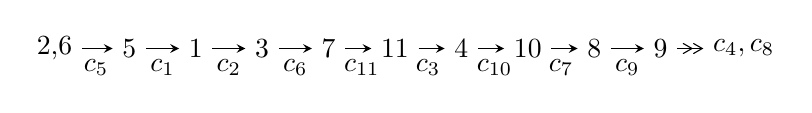
\begin{tikzpicture}[x=24pt, y=7pt]
	% node
	\node (A0) at (-1/8, 0) {2,6};
	\node (A1) at (1, 0) {5};
	\node (A2) at (2, 0) {1};
	\node (A3) at (3, 0) {3};
	\node (A4) at (4, 0) {7};
	\node (A5) at (5, 0) {11};
	\node (A6) at (6, 0) {4};
	\node (A7) at (7, 0) {10};
	\node (A8) at (8, 0) {8};
	\node (A9) at (9, 0) {9};
	\node (C1) at (1/2, -1) {$c_{5}$};
	\node (C2) at (3/2, -1) {$c_{1}$};
	\node (C3) at (5/2, -1) {$c_{2}$};
	\node (C4) at (7/2, -1) {$c_{6}$};
	\node (C5) at (9/2, -1) {$c_{11}$};
	\node (C6) at (11/2, -1) {$c_{3}$};
	\node (C7) at (13/2, -1) {$c_{10}$};
	\node (C8) at (15/2, -1) {$c_{7}$};
	\node (C9) at (17/2, -1) {$c_{9}$};
	\node (A10) at (41/4, 0) {$c_{4},c_{8}$};

	% edge
	\draw[->,>=stealth]	
	(A0) edge (A1) (A1) edge (A2) (A2) edge (A3) (A3) edge (A4) (A4) edge (A5) (A5) edge (A6) (A6) edge (A7) (A7) edge (A8) (A8) edge (A9) ;
	\draw[->>,>={angle 60}]	
	(A9) edge (A10);
\end{tikzpicture} \\ 

\end{tabular} \\

\footnotetext{
The image of knot diagram is generated by the software ``\textbf{Draw programme}" developed by Andrew Bartholomew(\url{http://www.layer8.co.uk/maths/draw/index.htm\#Running-draw}), where we modified some parts for our purpose(\url{https://github.com/CATsTAILs/LinksPainter}).
}\phantom \\ \newline 
\centering \textbf{Ideals for irreducible components\footnotemark of $X_{\text{par}}$} 
 
\begin{align*}
I^u_{1}&=\langle 
u^{53}- u^{52}+\cdots+3 u-1\rangle \\
\\
\end{align*}
\raggedright * 1 irreducible components of $\dim_{\mathbb{C}}=0$, with total 53 representations.\\
\footnotetext{All coefficients of polynomials are rational numbers. But the coefficients are sometimes approximated in decimal forms when there is not enough margin.}
\newpage
\renewcommand{\arraystretch}{1}
\centering \section*{I. $I^u_{1}= \langle u^{53}- u^{52}+\cdots+3 u-1 \rangle$}
\flushleft \textbf{(i) Arc colorings}\\
\begin{tabular}{m{7pt} m{180pt} m{7pt} m{180pt} }
\flushright $a_{2}=$&$\begin{pmatrix}0\\u\end{pmatrix}$ \\
\flushright $a_{6}=$&$\begin{pmatrix}1\\0\end{pmatrix}$ \\
\flushright $a_{5}=$&$\begin{pmatrix}1\\- u^2\end{pmatrix}$ \\
\flushright $a_{1}=$&$\begin{pmatrix}u\\- u^3+u\end{pmatrix}$ \\
\flushright $a_{3}=$&$\begin{pmatrix}- u^3\\u^5- u^3+u\end{pmatrix}$ \\
\flushright $a_{7}=$&$\begin{pmatrix}u^8- u^6+u^4+1\\- u^{10}+2 u^8-3 u^6+2 u^4- u^2\end{pmatrix}$ \\
\flushright $a_{11}=$&$\begin{pmatrix}u^3\\- u^3+u\end{pmatrix}$ \\
\flushright $a_{4}=$&$\begin{pmatrix}u^{11}-2 u^9+2 u^7- u^3\\- u^{11}+3 u^9-4 u^7+3 u^5- u^3+u\end{pmatrix}$ \\
\flushright $a_{10}=$&$\begin{pmatrix}u^{21}-4 u^{19}+9 u^{17}-12 u^{15}+12 u^{13}-10 u^{11}+9 u^9-6 u^7+3 u^5+u\\- u^{23}+5 u^{21}+\cdots-2 u^3+u\end{pmatrix}$ \\
\flushright $a_{8}=$&$\begin{pmatrix}u^{34}-7 u^{32}+\cdots+u^2+1\\- u^{36}+8 u^{34}+\cdots+4 u^6- u^4\end{pmatrix}$ \\
\flushright $a_{9}=$&$\begin{pmatrix}u^{47}-10 u^{45}+\cdots+4 u^5+2 u\\- u^{49}+11 u^{47}+\cdots-2 u^3+u\end{pmatrix}$\\ \flushright $a_{9}=$&$\begin{pmatrix}u^{47}-10 u^{45}+\cdots+4 u^5+2 u\\- u^{49}+11 u^{47}+\cdots-2 u^3+u\end{pmatrix}$\\&\end{tabular}
\flushleft \textbf{(ii) Obstruction class $= -1$}\\~\\
\flushleft \textbf{(iii) Cusp Shapes $= -4 u^{52}+52 u^{50}+\cdots+12 u-14$}\\~\\
\newpage\renewcommand{\arraystretch}{1}
\flushleft \textbf{(iv) u-Polynomials at the component}\newline \\
\begin{tabular}{m{50pt}|m{274pt}}
Crossings & \hspace{64pt}u-Polynomials at each crossing \\
\hline $$\begin{aligned}c_{1},c_{5}\end{aligned}$$&$\begin{aligned}
&u^{53}+u^{52}+\cdots+3 u+1
\end{aligned}$\\
\hline $$\begin{aligned}c_{2}\end{aligned}$$&$\begin{aligned}
&u^{53}+25 u^{52}+\cdots+3 u+1
\end{aligned}$\\
\hline $$\begin{aligned}c_{3}\end{aligned}$$&$\begin{aligned}
&u^{53}+7 u^{52}+\cdots+41 u+5
\end{aligned}$\\
\hline $$\begin{aligned}c_{4},c_{8}\end{aligned}$$&$\begin{aligned}
&u^{53}- u^{52}+\cdots+u+1
\end{aligned}$\\
\hline $$\begin{aligned}c_{6}\end{aligned}$$&$\begin{aligned}
&u^{53}- u^{52}+\cdots+149 u+97
\end{aligned}$\\
\hline $$\begin{aligned}c_{7},c_{9},c_{10}\end{aligned}$$&$\begin{aligned}
&u^{53}+13 u^{52}+\cdots+3 u+1
\end{aligned}$\\
\hline $$\begin{aligned}c_{11}\end{aligned}$$&$\begin{aligned}
&u^{53}+3 u^{52}+\cdots+213 u+39
\end{aligned}$\\
\hline
\end{tabular}\\~\\
\newpage\renewcommand{\arraystretch}{1}
\flushleft \textbf{(v) Riley Polynomials at the component}\newline \\
\begin{tabular}{m{50pt}|m{274pt}}
Crossings & \hspace{64pt}Riley Polynomials at each crossing \\
\hline $$\begin{aligned}c_{1},c_{5}\end{aligned}$$&$\begin{aligned}
&y^{53}-25 y^{52}+\cdots+3 y-1
\end{aligned}$\\
\hline $$\begin{aligned}c_{2}\end{aligned}$$&$\begin{aligned}
&y^{53}+7 y^{52}+\cdots+3 y-1
\end{aligned}$\\
\hline $$\begin{aligned}c_{3}\end{aligned}$$&$\begin{aligned}
&y^{53}-5 y^{52}+\cdots+911 y-25
\end{aligned}$\\
\hline $$\begin{aligned}c_{4},c_{8}\end{aligned}$$&$\begin{aligned}
&y^{53}-13 y^{52}+\cdots+3 y-1
\end{aligned}$\\
\hline $$\begin{aligned}c_{6}\end{aligned}$$&$\begin{aligned}
&y^{53}-17 y^{52}+\cdots+199323 y-9409
\end{aligned}$\\
\hline $$\begin{aligned}c_{7},c_{9},c_{10}\end{aligned}$$&$\begin{aligned}
&y^{53}+55 y^{52}+\cdots-5 y-1
\end{aligned}$\\
\hline $$\begin{aligned}c_{11}\end{aligned}$$&$\begin{aligned}
&y^{53}+11 y^{52}+\cdots-28185 y-1521
\end{aligned}$\\
\hline
\end{tabular}\\~\\
\newpage\flushleft \textbf{(vi) Complex Volumes and Cusp Shapes}
$$\begin{array}{c|c|c}  
\text{Solutions to }I^u_{1}& \I (\text{vol} + \sqrt{-1}CS) & \text{Cusp shape}\\
 \hline 
\begin{aligned}
u &= \phantom{-}1.044500 + 0.281512 I\end{aligned}
 & -2.20764 - 0.64085 I & -5.73049 + 0.77381 I \\ \hline\begin{aligned}
u &= \phantom{-}1.044500 - 0.281512 I\end{aligned}
 & -2.20764 + 0.64085 I & -5.73049 - 0.77381 I \\ \hline\begin{aligned}
u &= \phantom{-}0.601217 + 0.686706 I\end{aligned}
 & \phantom{-}8.50588 - 6.50884 I & \phantom{-}1.27031 + 5.73425 I \\ \hline\begin{aligned}
u &= \phantom{-}0.601217 - 0.686706 I\end{aligned}
 & \phantom{-}8.50588 + 6.50884 I & \phantom{-}1.27031 - 5.73425 I \\ \hline\begin{aligned}
u &= \phantom{-}0.974822 + 0.492221 I\end{aligned}
 & -0.225106 - 0.871265 I & -4.08839 - 0.80386 I \\ \hline\begin{aligned}
u &= \phantom{-}0.974822 - 0.492221 I\end{aligned}
 & -0.225106 + 0.871265 I & -4.08839 + 0.80386 I \\ \hline\begin{aligned}
u &= -0.586774 + 0.690510 I\end{aligned}
 & \phantom{-}8.78157 + 0.18779 I & \phantom{-}1.88251 - 0.64861 I \\ \hline\begin{aligned}
u &= -0.586774 - 0.690510 I\end{aligned}
 & \phantom{-}8.78157 - 0.18779 I & \phantom{-}1.88251 + 0.64861 I \\ \hline\begin{aligned}
u &= \phantom{-}1.109660 + 0.186764 I\end{aligned}
 & \phantom{-}2.94416 + 0.20510 I & -5.58587 + 0.61243 I \\ \hline\begin{aligned}
u &= \phantom{-}1.109660 - 0.186764 I\end{aligned}
 & \phantom{-}2.94416 - 0.20510 I & -5.58587 - 0.61243 I \\ \hline\begin{aligned}
u &= -1.102420 + 0.258443 I\end{aligned}
 & -4.56669 - 2.49112 I & -11.89781 + 4.18392 I \\ \hline\begin{aligned}
u &= -1.102420 - 0.258443 I\end{aligned}
 & -4.56669 + 2.49112 I & -11.89781 - 4.18392 I \\ \hline\begin{aligned}
u &= -1.122120 + 0.196280 I\end{aligned}
 & \phantom{-}2.54225 - 6.40452 I & -6.41624 + 4.33917 I \\ \hline\begin{aligned}
u &= -1.122120 - 0.196280 I\end{aligned}
 & \phantom{-}2.54225 + 6.40452 I & -6.41624 - 4.33917 I \\ \hline\begin{aligned}
u &= \phantom{-}0.971931 + 0.595508 I\end{aligned}
 & \phantom{-}7.41049 + 1.56089 I & \phantom{-0.000000 } 0 \\ \hline\begin{aligned}
u &= \phantom{-}0.971931 - 0.595508 I\end{aligned}
 & \phantom{-}7.41049 - 1.56089 I & \phantom{-0.000000 } 0 \\ \hline\begin{aligned}
u &= \phantom{-}0.366014 + 0.773541 I\end{aligned}
 & \phantom{-}7.29360 + 8.95041 I & -0.09124 - 5.62138 I \\ \hline\begin{aligned}
u &= \phantom{-}0.366014 - 0.773541 I\end{aligned}
 & \phantom{-}7.29360 - 8.95041 I & -0.09124 + 5.62138 I \\ \hline\begin{aligned}
u &= -0.376178 + 0.768520 I\end{aligned}
 & \phantom{-}7.69936 - 2.64631 I & \phantom{-}0.774092 + 0.704677 I \\ \hline\begin{aligned}
u &= -0.376178 - 0.768520 I\end{aligned}
 & \phantom{-}7.69936 + 2.64631 I & \phantom{-}0.774092 - 0.704677 I \\ \hline\begin{aligned}
u &= -1.098220 + 0.328717 I\end{aligned}
 & -5.25608 + 2.82044 I & -13.7464 - 4.6104 I \\ \hline\begin{aligned}
u &= -1.098220 - 0.328717 I\end{aligned}
 & -5.25608 - 2.82044 I & -13.7464 + 4.6104 I \\ \hline\begin{aligned}
u &= -0.983871 + 0.595556 I\end{aligned}
 & \phantom{-}7.60812 + 4.77001 I & \phantom{-0.000000 } 0. - 5.11123 I \\ \hline\begin{aligned}
u &= -0.983871 - 0.595556 I\end{aligned}
 & \phantom{-}7.60812 - 4.77001 I & \phantom{-0.000000 -}0. + 5.11123 I \\ \hline\begin{aligned}
u &= \phantom{-}0.592887 + 0.582181 I\end{aligned}
 & \phantom{-}0.88261 - 3.44954 I & -2.55100 + 7.40984 I \\ \hline\begin{aligned}
u &= \phantom{-}0.592887 - 0.582181 I\end{aligned}
 & \phantom{-}0.88261 + 3.44954 I & -2.55100 - 7.40984 I \\ \hline\begin{aligned}
u &= -1.038830 + 0.540274 I\end{aligned}
 & \phantom{-}0.66178 + 4.72185 I & \phantom{-0.000000 } 0. - 6.22617 I \\ \hline\begin{aligned}
u &= -1.038830 - 0.540274 I\end{aligned}
 & \phantom{-}0.66178 - 4.72185 I & \phantom{-0.000000 -}0. + 6.22617 I \\ \hline\begin{aligned}
u &= \phantom{-}1.108380 + 0.429410 I\end{aligned}
 & \phantom{-}0.525380 - 0.893417 I & -6.66537 + 0. I\phantom{ +0.000000I} \\ \hline\begin{aligned}
u &= \phantom{-}1.108380 - 0.429410 I\end{aligned}
 & \phantom{-}0.525380 + 0.893417 I & -6.66537 + 0. I\phantom{ +0.000000I}\\
 \hline 
 \end{array}$$\newpage$$\begin{array}{c|c|c}  
\text{Solutions to }I^u_{1}& \I (\text{vol} + \sqrt{-1}CS) & \text{Cusp shape}\\
 \hline 
\begin{aligned}
u &= -1.117790 + 0.404581 I\end{aligned}
 & \phantom{-}0.34604 + 6.68644 I & -7.28464 - 6.64124 I \\ \hline\begin{aligned}
u &= -1.117790 - 0.404581 I\end{aligned}
 & \phantom{-}0.34604 - 6.68644 I & -7.28464 + 6.64124 I \\ \hline\begin{aligned}
u &= \phantom{-}0.332464 + 0.722196 I\end{aligned}
 & -0.29834 + 5.13851 I & -4.80621 - 6.56976 I \\ \hline\begin{aligned}
u &= \phantom{-}0.332464 - 0.722196 I\end{aligned}
 & -0.29834 - 5.13851 I & -4.80621 + 6.56976 I \\ \hline\begin{aligned}
u &= -0.491709 + 0.618554 I\end{aligned}
 & \phantom{-}2.27338 - 0.13836 I & \phantom{-}2.37846 + 0.39315 I \\ \hline\begin{aligned}
u &= -0.491709 - 0.618554 I\end{aligned}
 & \phantom{-}2.27338 + 0.13836 I & \phantom{-}2.37846 - 0.39315 I \\ \hline\begin{aligned}
u &= -0.378665 + 0.682475 I\end{aligned}
 & \phantom{-}1.76473 - 1.60253 I & \phantom{-}1.33859 + 1.09595 I \\ \hline\begin{aligned}
u &= -0.378665 - 0.682475 I\end{aligned}
 & \phantom{-}1.76473 + 1.60253 I & \phantom{-}1.33859 - 1.09595 I \\ \hline\begin{aligned}
u &= \phantom{-}1.102860 + 0.521380 I\end{aligned}
 & -3.95438 - 4.57454 I & \phantom{-0.000000 } 0 \\ \hline\begin{aligned}
u &= \phantom{-}1.102860 - 0.521380 I\end{aligned}
 & -3.95438 + 4.57454 I & \phantom{-0.000000 } 0 \\ \hline\begin{aligned}
u &= -1.093000 + 0.554934 I\end{aligned}
 & -0.31357 + 6.39150 I & \phantom{-0.000000 } 0 \\ \hline\begin{aligned}
u &= -1.093000 - 0.554934 I\end{aligned}
 & -0.31357 - 6.39150 I & \phantom{-0.000000 } 0 \\ \hline\begin{aligned}
u &= \phantom{-}1.114580 + 0.556654 I\end{aligned}
 & -2.57269 - 10.01430 I & \phantom{-0.000000 } 0 \\ \hline\begin{aligned}
u &= \phantom{-}1.114580 - 0.556654 I\end{aligned}
 & -2.57269 + 10.01430 I & \phantom{-0.000000 } 0 \\ \hline\begin{aligned}
u &= -1.114170 + 0.582898 I\end{aligned}
 & \phantom{-}5.52079 + 7.74501 I & \phantom{-0.000000 } 0 \\ \hline\begin{aligned}
u &= -1.114170 - 0.582898 I\end{aligned}
 & \phantom{-}5.52079 - 7.74501 I & \phantom{-0.000000 } 0 \\ \hline\begin{aligned}
u &= \phantom{-}1.119280 + 0.581631 I\end{aligned}
 & \phantom{-}5.0695 - 14.0551 I & \phantom{-0.000000 } 0 \\ \hline\begin{aligned}
u &= \phantom{-}1.119280 - 0.581631 I\end{aligned}
 & \phantom{-}5.0695 + 14.0551 I & \phantom{-0.000000 } 0 \\ \hline\begin{aligned}
u &= \phantom{-}0.262528 + 0.616219 I\end{aligned}
 & -1.62999 + 0.09542 I & -8.49556 + 0.70141 I \\ \hline\begin{aligned}
u &= \phantom{-}0.262528 - 0.616219 I\end{aligned}
 & -1.62999 - 0.09542 I & -8.49556 - 0.70141 I \\ \hline\begin{aligned}
u &= \phantom{-}0.022954 + 0.641795 I\end{aligned}
 & \phantom{-}3.51831 - 2.96655 I & -2.71846 + 2.72944 I \\ \hline\begin{aligned}
u &= \phantom{-}0.022954 - 0.641795 I\end{aligned}
 & \phantom{-}3.51831 + 2.96655 I & -2.71846 - 2.72944 I \\ \hline\begin{aligned}
u &= \phantom{-}0.559370\phantom{ +0.000000I}\end{aligned}
 & -1.01608\phantom{ +0.000000I} & -9.59730\phantom{ +0.000000I}\\
 \hline 
 \end{array}$$\newpage
\newpage\renewcommand{\arraystretch}{1}
\centering \section*{ II. u-Polynomials}
\begin{tabular}{m{50pt}|m{274pt}}
Crossings & \hspace{64pt}u-Polynomials at each crossing \\
\hline $$\begin{aligned}c_{1},c_{5}\end{aligned}$$&$\begin{aligned}
&u^{53}+u^{52}+\cdots+3 u+1
\end{aligned}$\\
\hline $$\begin{aligned}c_{2}\end{aligned}$$&$\begin{aligned}
&u^{53}+25 u^{52}+\cdots+3 u+1
\end{aligned}$\\
\hline $$\begin{aligned}c_{3}\end{aligned}$$&$\begin{aligned}
&u^{53}+7 u^{52}+\cdots+41 u+5
\end{aligned}$\\
\hline $$\begin{aligned}c_{4},c_{8}\end{aligned}$$&$\begin{aligned}
&u^{53}- u^{52}+\cdots+u+1
\end{aligned}$\\
\hline $$\begin{aligned}c_{6}\end{aligned}$$&$\begin{aligned}
&u^{53}- u^{52}+\cdots+149 u+97
\end{aligned}$\\
\hline $$\begin{aligned}c_{7},c_{9},c_{10}\end{aligned}$$&$\begin{aligned}
&u^{53}+13 u^{52}+\cdots+3 u+1
\end{aligned}$\\
\hline $$\begin{aligned}c_{11}\end{aligned}$$&$\begin{aligned}
&u^{53}+3 u^{52}+\cdots+213 u+39
\end{aligned}$\\
\hline
\end{tabular}\newpage\renewcommand{\arraystretch}{1}
\centering \section*{ III. Riley Polynomials}
\begin{tabular}{m{50pt}|m{274pt}}
Crossings & \hspace{64pt}Riley Polynomials at each crossing \\
\hline $$\begin{aligned}c_{1},c_{5}\end{aligned}$$&$\begin{aligned}
&y^{53}-25 y^{52}+\cdots+3 y-1
\end{aligned}$\\
\hline $$\begin{aligned}c_{2}\end{aligned}$$&$\begin{aligned}
&y^{53}+7 y^{52}+\cdots+3 y-1
\end{aligned}$\\
\hline $$\begin{aligned}c_{3}\end{aligned}$$&$\begin{aligned}
&y^{53}-5 y^{52}+\cdots+911 y-25
\end{aligned}$\\
\hline $$\begin{aligned}c_{4},c_{8}\end{aligned}$$&$\begin{aligned}
&y^{53}-13 y^{52}+\cdots+3 y-1
\end{aligned}$\\
\hline $$\begin{aligned}c_{6}\end{aligned}$$&$\begin{aligned}
&y^{53}-17 y^{52}+\cdots+199323 y-9409
\end{aligned}$\\
\hline $$\begin{aligned}c_{7},c_{9},c_{10}\end{aligned}$$&$\begin{aligned}
&y^{53}+55 y^{52}+\cdots-5 y-1
\end{aligned}$\\
\hline $$\begin{aligned}c_{11}\end{aligned}$$&$\begin{aligned}
&y^{53}+11 y^{52}+\cdots-28185 y-1521
\end{aligned}$\\
\hline
\end{tabular}
\vskip 2pc
\end{document}